
\documentclass[border=10pt, 12pt]{standalone}
\usepackage[svgnames]{xcolor}
\usepackage{amsmath}
\usepackage{pgfplots}
\pgfplotsset{compat=newest}
\usepackage[sfdefault]{FiraSans}
\usepackage{FiraMono}
\renewcommand*\familydefault{\sfdefault}
\begin{document}
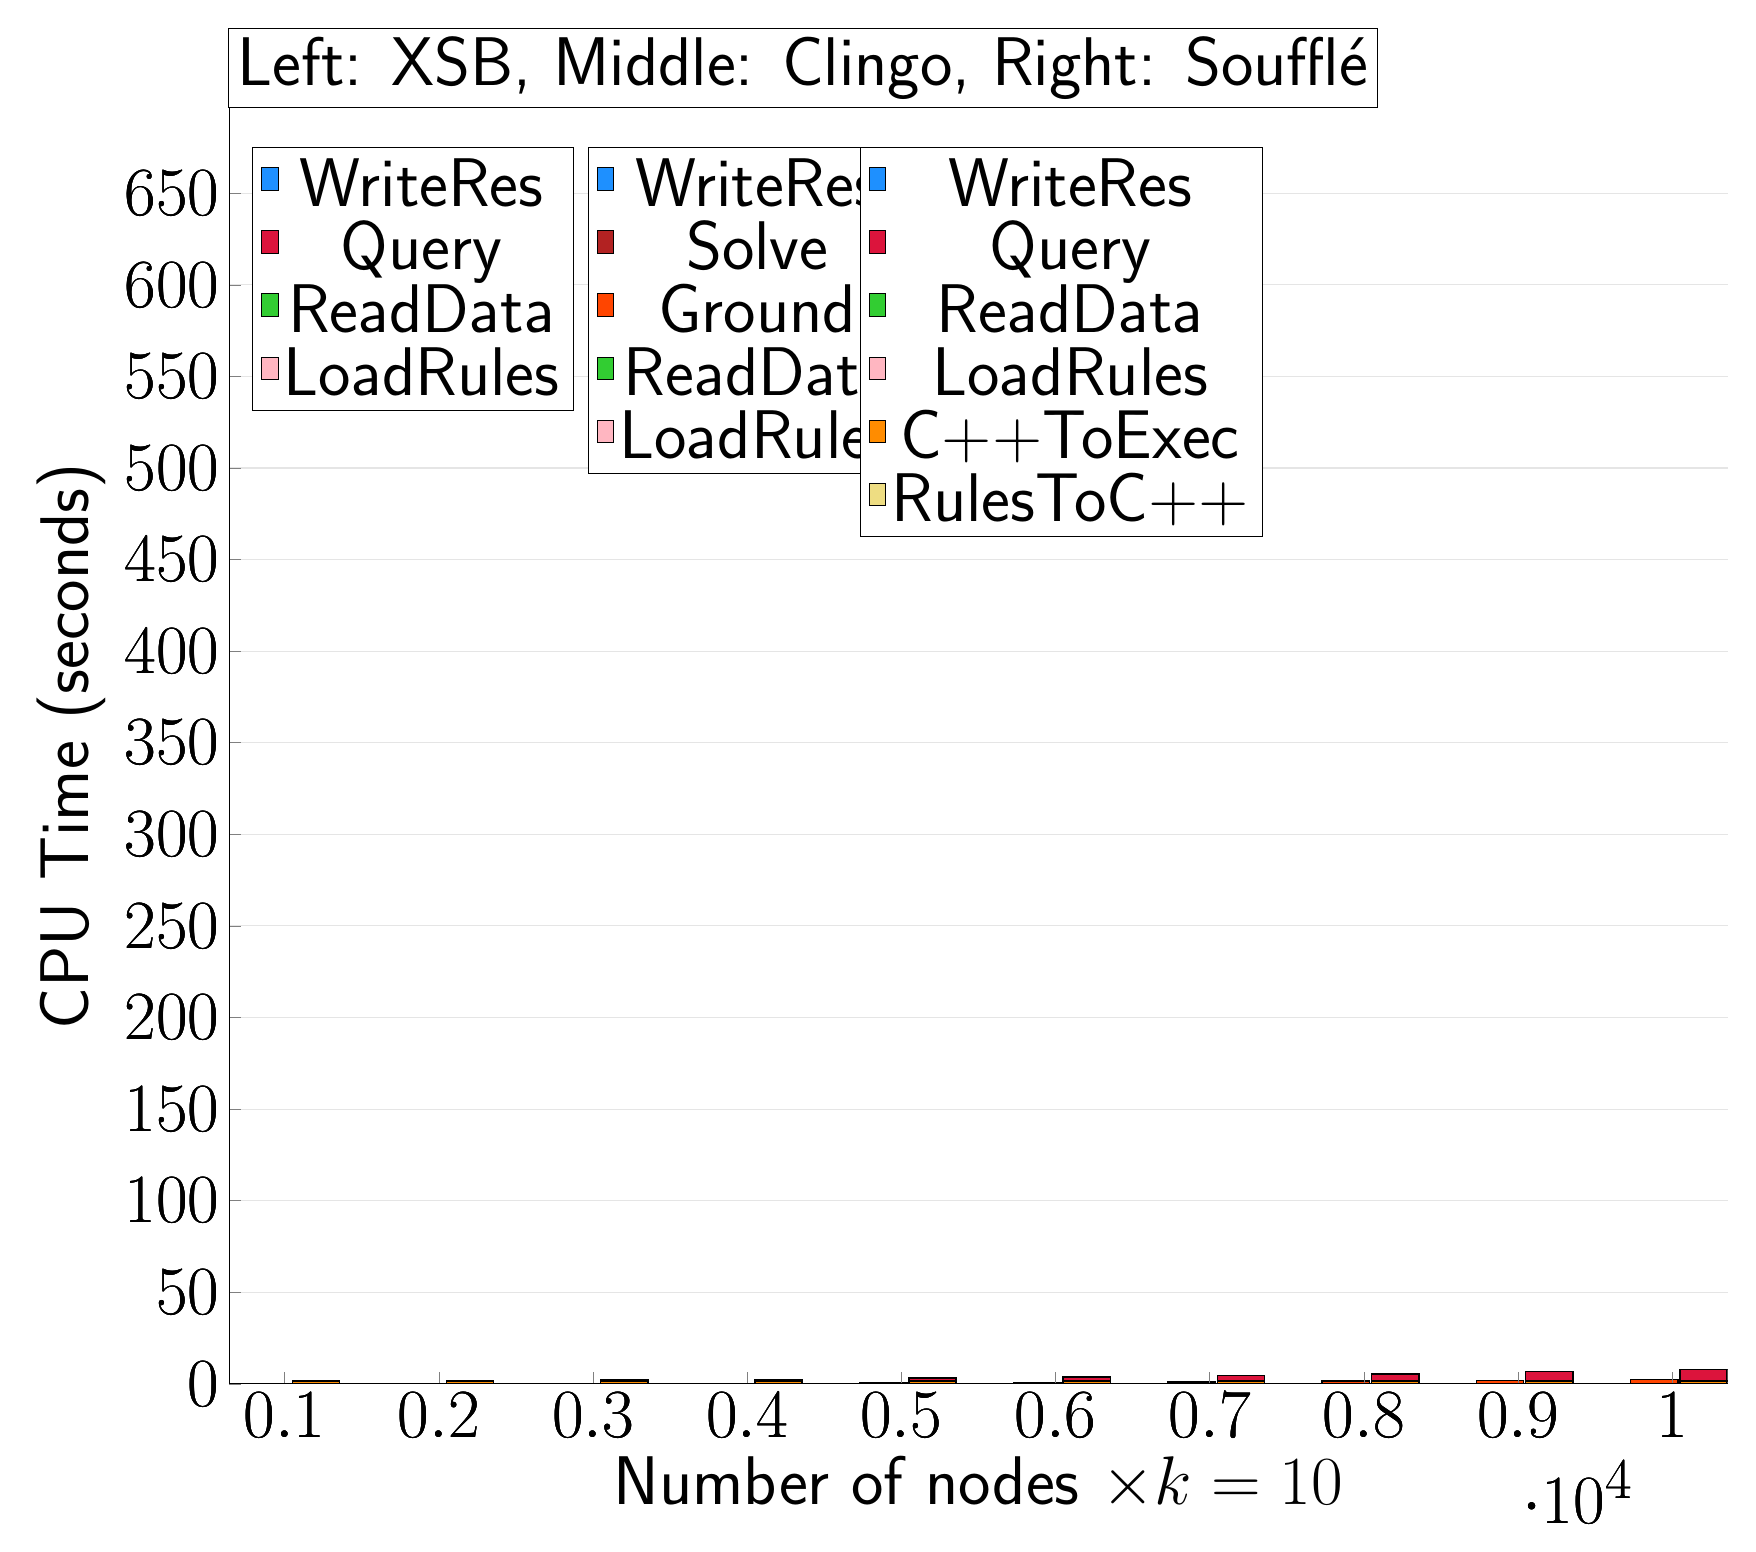
\begin{tikzpicture}
                        \begin{axis}[bar shift=-24.3pt, 
   ybar stacked,
   width=1.7\textwidth,
   bar width=0.6cm,
   ymajorgrids, tick align=inside,
   major grid style={draw=gray!20},
   xtick=data,
   ymin=0, ymax=696.3414,
   axis x line*=bottom,
   axis y line*=left,
   enlarge x limits=0.04,
   legend style={
       at={(0.23, 0.97)},
       anchor=north east,
       legend columns=1,
       font=\Huge,
   },
   ylabel={CPU Time (seconds)},
   xlabel={Number of nodes $\times k=10$},
   label style={font=\Huge},
   tick label style={font=\Huge},
]
\addlegendimage{fill=DodgerBlue, draw=black, line width=0.2pt}
\addlegendentry{WriteRes}
\addlegendimage{fill=Crimson, draw=black, line width=0.2pt}
\addlegendentry{Query}
\addlegendimage{fill=LimeGreen, draw=black, line width=0.2pt}
\addlegendentry{ReadData}
\addlegendimage{fill=LightPink, draw=black, line width=0.2pt}
\addlegendentry{LoadRules}
\addplot +[fill=LightPink, draw=black, line width=0.55pt] coordinates {
(1000, 0.0005526000000000001)
(2000, 0.0005547999999999996)
(3000, 0.0005532000000000002)
(4000, 0.0005625999999999997)
(5000, 0.0005537999999999999)
(6000, 0.0005533999999999996)
(7000, 0.0005569999999999998)
(8000, 0.0005493999999999996)
(9000, 0.0005657999999999998)
(10000, 0.0005647999999999999)
};
\addplot +[fill=LimeGreen, draw=black, line width=0.55pt] coordinates {
(1000, 0.0008986)
(2000, 0.0017276)
(3000, 0.002535)
(4000, 0.0033836000000000005)
(5000, 0.0042334)
(6000, 0.005056799999999999)
(7000, 0.0058628)
(8000, 0.0066678)
(9000, 0.0075066)
(10000, 0.0083852)
};
\addplot +[fill=Crimson, draw=black, line width=0.55pt] coordinates {
(1000, 2.000000000000022e-05)
(2000, 2.979999999999996e-05)
(3000, 4.140000000000048e-05)
(4000, 5.2800000000000775e-05)
(5000, 6.51999999999986e-05)
(6000, 7.93999999999989e-05)
(7000, 8.519999999999917e-05)
(8000, 9.840000000000113e-05)
(9000, 0.0001114000000000004)
(10000, 0.00013139999999999978)
};
\addplot +[fill=DodgerBlue, draw=black, line width=0.55pt] coordinates {
(1000, 9.400000000000018e-05)
(2000, 0.00012419999999999966)
(3000, 0.00015499999999999932)
(4000, 0.00019259999999999904)
(5000, 0.000219000000000001)
(6000, 0.0002480000000000011)
(7000, 0.00028400000000000067)
(8000, 0.00030879999999999867)
(9000, 0.000349)
(10000, 0.0003761999999999994)
};
\end{axis}

\begin{axis}[bar shift=-6.5pt, 
   ybar stacked,
   width=1.7\textwidth,
   bar width=0.6cm,
   ymajorgrids, tick align=inside,
   major grid style={draw=none},
   xtick=data,
   ymin=0, ymax=696.3414,
   axis x line*=none,
   axis y line*=none,
   enlarge x limits=0.04,
   legend style={
       at={(0.454, 0.97)},
       anchor=north east,
       legend columns=1,
       font=\Huge,
   },
   label style={font=\Huge},
   tick label style={font=\Huge},
]
\addlegendimage{fill=DodgerBlue, draw=black, line width=0.2pt}
\addlegendentry{WriteRes}
\addlegendimage{fill=FireBrick, draw=black, line width=0.2pt}
\addlegendentry{Solve}
\addlegendimage{fill=OrangeRed, draw=black, line width=0.2pt}
\addlegendentry{Ground}
\addlegendimage{fill=LimeGreen, draw=black, line width=0.2pt}
\addlegendentry{ReadData}
\addlegendimage{fill=LightPink, draw=black, line width=0.2pt}
\addlegendentry{LoadRules}
\addplot +[fill=LightPink, draw=black, line width=0.55pt] coordinates {
(1000, 0.0)
(2000, 0.0)
(3000, 0.0)
(4000, 0.0)
(5000, 0.0)
(6000, 0.0)
(7000, 0.0)
(8000, 0.0)
(9000, 0.0)
(10000, 0.0)
};
\addplot +[fill=LimeGreen, draw=black, line width=0.55pt] coordinates {
(1000, 0.0)
(2000, 0.0)
(3000, 0.010000000000000009)
(4000, 0.010000000000000009)
(5000, 0.010000000000000009)
(6000, 0.010000000000000009)
(7000, 0.010000000000000009)
(8000, 0.020000000000000018)
(9000, 0.020000000000000018)
(10000, 0.020000000000000018)
};
\addplot +[fill=OrangeRed, draw=black, line width=0.55pt] coordinates {
(1000, 0.020000000000000018)
(2000, 0.07)
(3000, 0.16000000000000003)
(4000, 0.29400000000000004)
(5000, 0.502)
(6000, 0.742)
(7000, 1.0459999999999998)
(8000, 1.378)
(9000, 1.86)
(10000, 2.272)
};
\addplot +[fill=FireBrick, draw=black, line width=0.55pt] coordinates {
(1000, 0.0)
(2000, 0.0)
(3000, 0.0)
(4000, 0.0040000000000000036)
(5000, 0.006000000000000005)
(6000, 0.008000000000000007)
(7000, 0.016000000000000014)
(8000, 0.020000000000000018)
(9000, 0.022000000000000065)
(10000, 0.025999999999999978)
};
\addplot +[fill=DodgerBlue, draw=black, line width=0.55pt] coordinates {
(1000, 0.0)
(2000, 0.0)
(3000, 0.0)
(4000, -0.0020000000000000018)
(5000, -0.006000000000000005)
(6000, -0.006000000000000005)
(7000, -0.016000000000000014)
(8000, -0.020000000000000018)
(9000, -0.022000000000000065)
(10000, -0.02399999999999993)
};
\end{axis}

\begin{axis}[bar shift=11.3pt, 
   ybar stacked,
   width=1.7\textwidth,
   bar width=0.6cm,
   ymajorgrids, tick align=inside,
   major grid style={draw=none},
   xtick=data,
   ymin=0, ymax=696.3414,
   axis x line*=none,
   axis y line*=none,
   enlarge x limits=0.04,
   legend style={
       at={(0.69, 0.97)},
       anchor=north east,
       legend columns=1,
       font=\Huge,
   },
   label style={font=\Huge},
   tick label style={font=\Huge},
]
\addlegendimage{fill=DodgerBlue, draw=black, line width=0.2pt}
\addlegendentry{WriteRes}
\addlegendimage{fill=Crimson, draw=black, line width=0.2pt}
\addlegendentry{Query}
\addlegendimage{fill=LimeGreen, draw=black, line width=0.2pt}
\addlegendentry{ReadData}
\addlegendimage{fill=LightPink, draw=black, line width=0.2pt}
\addlegendentry{LoadRules}
\addlegendimage{fill=DarkOrange, draw=black, line width=0.2pt}
\addlegendentry{C++ToExec}
\addlegendimage{fill=LightGoldenrod, draw=black, line width=0.2pt}
\addlegendentry{RulesToC++}
\addplot +[fill=LightGoldenrod, draw=black, line width=0.55pt] coordinates {
(1000, 0.008000000000000002)
(2000, 0.010000000000000002)
(3000, 0.010000000000000002)
(4000, 0.008000000000000002)
(5000, 0.008000000000000002)
(6000, 0.006000000000000001)
(7000, 0.006000000000000001)
(8000, 0.004000000000000001)
(9000, 0.008000000000000002)
(10000, 0.008000000000000002)
};
\addplot +[fill=DarkOrange, draw=black, line width=0.55pt] coordinates {
(1000, 1.512)
(2000, 1.524)
(3000, 1.5260000000000002)
(4000, 1.5260000000000002)
(5000, 1.5240000000000002)
(6000, 1.532)
(7000, 1.5320000000000003)
(8000, 1.52)
(9000, 1.52)
(10000, 1.522)
};
\addplot +[fill=LightPink, draw=black, line width=0.55pt] coordinates {
(1000, 0.00014680000000000002)
(2000, 0.00015700000000000002)
(3000, 0.0001438)
(4000, 0.0001374)
(5000, 0.000151)
(6000, 0.0001526)
(7000, 0.0001396)
(8000, 0.000146)
(9000, 0.00015160000000000003)
(10000, 0.00013059999999999998)
};
\addplot +[fill=LimeGreen, draw=black, line width=0.55pt] coordinates {
(1000, 0.0039578)
(2000, 0.0071868)
(3000, 0.008899)
(4000, 0.011774000000000001)
(5000, 0.013603200000000001)
(6000, 0.016727)
(7000, 0.0172266)
(8000, 0.019974600000000002)
(9000, 0.0229098)
(10000, 0.022459)
};
\addplot +[fill=Crimson, draw=black, line width=0.55pt] coordinates {
(1000, 0.06844999999999998)
(2000, 0.23149900000000004)
(3000, 0.5222436)
(4000, 0.9444616)
(5000, 1.494782)
(6000, 2.1751980000000004)
(7000, 2.999714)
(8000, 3.9550899999999998)
(9000, 5.051918)
(10000, 6.298533999999999)
};
\addplot +[fill=DodgerBlue, draw=black, line width=0.55pt] coordinates {
(1000, 0.00022040000000000002)
(2000, 0.000232)
(3000, 0.00025120000000000003)
(4000, 0.00027860000000000005)
(5000, 0.00029240000000000006)
(6000, 0.000335)
(7000, 0.0002846)
(8000, 0.0003522)
(9000, 0.0003836)
(10000, 0.00039880000000000004)
};
\end{axis}


\node[anchor=south, draw, fill=white] at (rel axis cs:0.42,1) {\Huge Left: XSB, Middle: Clingo, Right: Soufflé};
\end{tikzpicture}
\end{document}
                    